\hypertarget{the-peripheral-nervous-system}{%
\chapter{The Peripheral Nervous System}\label{the-peripheral-nervous-system}}

The peripheral nervous system (PNS) is one of two components that make up the nervous system of bilateral animals, with the other part being the central nervous system (CNS). The PNS consists of the nerves and ganglia outside the brain and spinal cord. The main function of the PNS is to connect the CNS to the limbs and organs, essentially serving as a relay between the brain and spinal cord and the rest of the body. Unlike the CNS, the PNS is not protected by the vertebral column and skull, or by the blood--brain barrier, which leaves it exposed to toxins and mechanical injuries.

The peripheral nervous system is divided into the somatic nervous system and the autonomic nervous system. In the somatic nervous system, the cranial nerves are part of the PNS with the exception of the optic nerve (cranial nerve II), along with the retina. The second cranial nerve is not a true peripheral nerve but a tract of the diencephalon. Cranial nerve ganglia originated in the CNS. However, the remaining ten cranial nerve axons extend beyond the brain and are therefore considered part of the PNS. The autonomic nervous system exerts involuntary control over smooth muscle and glands. The connection between CNS and organs allows the system to be in two different functional states: sympathetic and parasympathetic.

The somatic nervous system is under voluntary control, and transmits signals from the brain to end organs such as muscles. The sensory nervous system is part of the somatic nervous system and transmits signals from senses such as taste and touch (including fine touch and gross touch) to the spinal cord and brain. The autonomic nervous system is a `self-regulating' system which influences the function of organs outside voluntary control, such as the heart rate, or the functions of the digestive system.

\hypertarget{the-somatic-nervous-system}{%
\section{The Somatic Nervous System}\label{the-somatic-nervous-system}}

The somatic nervous system includes the sensory neurons that convey information from the body to the CNS. The cell bodies of these sensory neurons lie in the dorsal root ganglia parallel to the spinal cord and in the cranial nerve ganglia.

In the head and neck, cranial nerves carry somatosensory data. There are twelve cranial nerves, ten of which originate from the brainstem, and mainly control the functions of the anatomic structures of the head with some exceptions. One unique cranial nerve is the vagus nerve, which receives sensory information from organs in the thorax and abdomen. The accessory nerve is responsible for innervating the sternocleidomastoid and trapezius muscles, neither of which being exclusively in the head.

\hypertarget{the-cranial-nerves}{%
\section{The Cranial Nerves}\label{the-cranial-nerves}}

Cranial nerves are the nerves that emerge directly from the brain (including the brainstem), of which there are conventionally considered twelve pairs. Cranial nerves relay information between the brain and parts of the body, primarily to and from regions of the head and neck, including the special senses of vision, taste, smell, and hearing.

The Graeco-Roman anatomist \href{https://en.wikipedia.org/wiki/Galen}{Galen} (AD 129--210) named seven pairs of cranial nerves. Much later, in 1664, English anatomist \href{https://en.wikipedia.org/wiki/Thomas_Willis}{Thomas Willis} suggested that there were actually 9 pairs of nerves. Finally, in 1778, German anatomist \href{https://en.wikipedia.org/wiki/Samuel_Thomas_von_Sömmerring}{Samuel Soemmering} named the 12 pairs of nerves that are generally accepted today.

The cranial nerves are considered components of the peripheral nervous system (PNS), although on a structural level the olfactory (I), optic (II), and trigeminal (V) nerves are more accurately considered part of the central nervous system (CNS).

The cranial nerves emerge from the central nervous system above the level of the first vertebrae of the vertebral column. Each cranial nerve is paired and is present on both sides. The numbering of the cranial nerves is based on the order in which they emerge from the brain and brainstem, from front to back. Most typically, humans are considered to have twelve pairs of cranial nerves (I--XII). The nerves are: the olfactory nerve (I), the optic nerve (II), oculomotor nerve (III), trochlear nerve (IV), trigeminal nerve (V), abducens nerve (VI), facial nerve (VII), vestibulocochlear nerve (VIII), glossopharyngeal nerve (IX), vagus nerve (X), accessory nerve (XI), and the hypoglossal nerve (XII).



\begin{figure}

{\centering 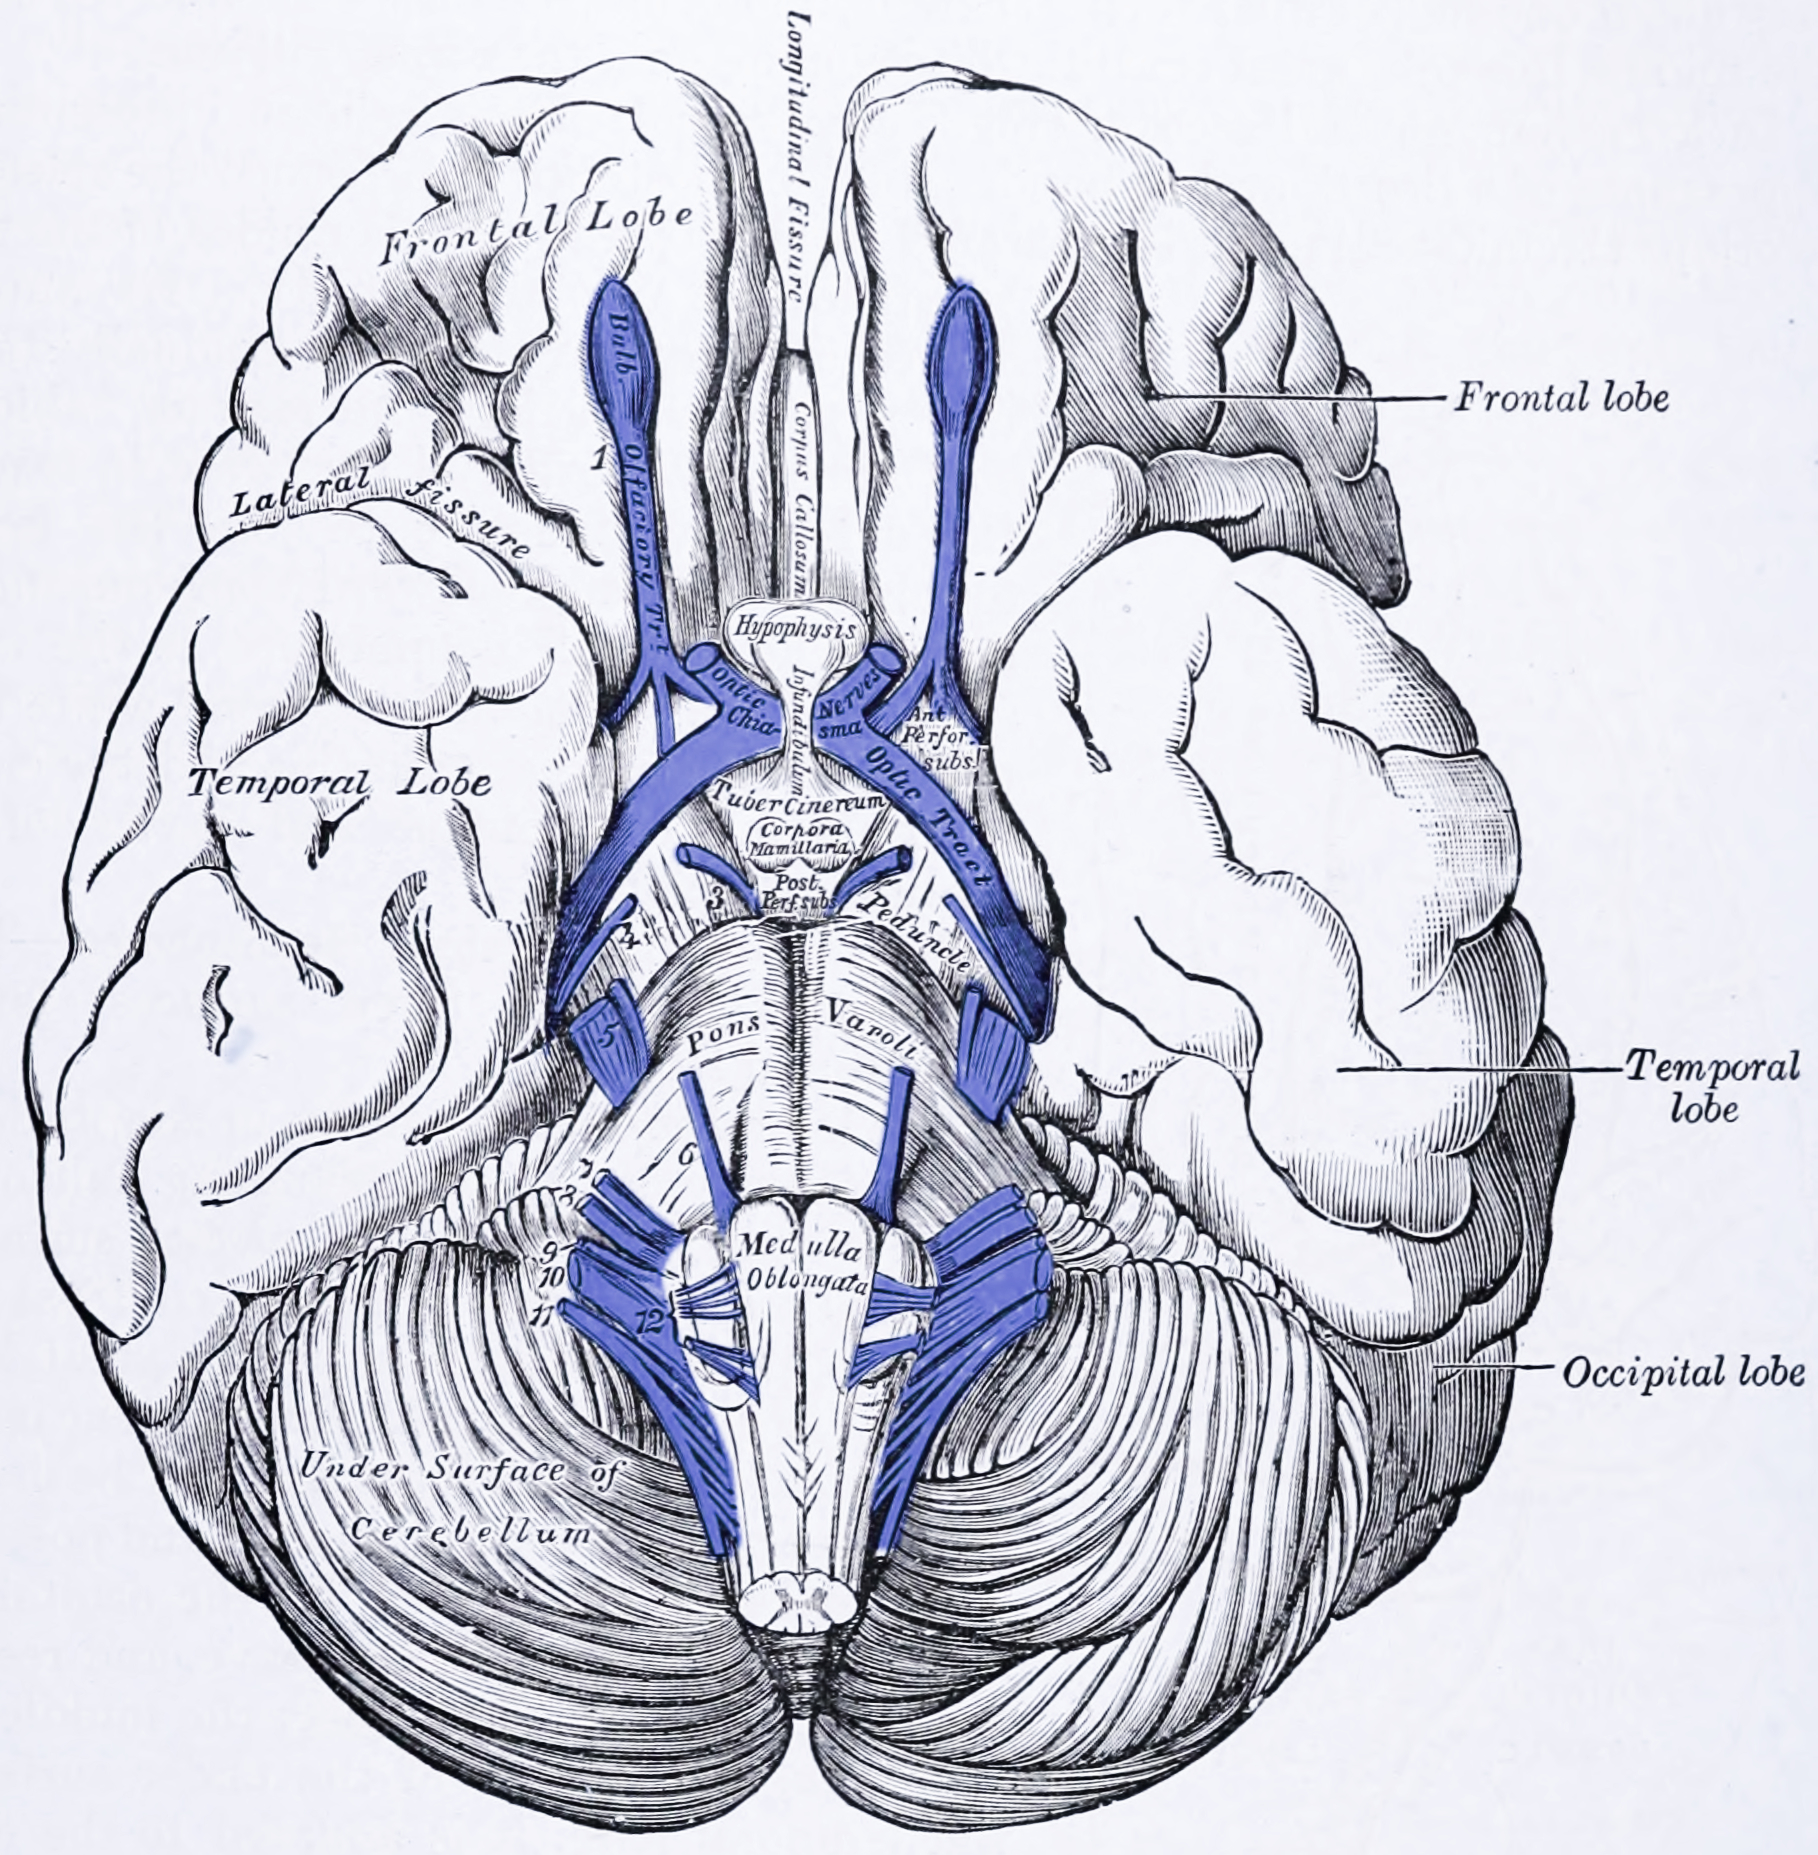
\includegraphics[width=0.7\linewidth]{./figures/pns/GrayAnat1918p817} 

}

\caption{View of the base of the brai. The cranial nerves are colored in purple and labeled with numbers on the left (1 to 12). From \href{https://archive.org/details/anatomyofhumanbo1918gray/page/n6/mode/2up}{Gray Henry, Anatomy of the Human Body. 20\textsuperscript{th} Edition, Lea \& Febiger, Philadelphia \& New York, 1918}}\label{fig:baseofbrain}
\end{figure}

With the exception of the olfactory nerve (I) and optic nerve (II), the cranial nerves emerge from the brainstem. The oculomotor nerve (III) and trochlear nerve (IV) emerge from the midbrain, the trigeminal (V), abducens (VI), facial (VII) and vestibulocochlea (VIII) from the pons, and the glossopharyngeal (IX), vagus (X), accessory (XI) and hypoglossal (XII) emerge from the medulla.

Grossly, all cranial nerves have a nucleus. With the exception of the olfactory nerve (I) and optic nerve (II), all the nuclei are present in the brainstem.

The midbrain of the brainstem has the nuclei of the oculomotor nerve (III) and trochlear nerve (IV); the pons has the nuclei of the trigeminal nerve (V), abducens nerve (VI), facial nerve (VII) and vestibulocochlear nerve (VIII); and the medulla has the nuclei of the glossopharyngeal nerve (IX), vagus nerve (X), accessory nerve (XI) and hypoglossal nerve (XII). The olfactory nerve (I) emerges from the olfactory bulb, and the optic nerve (II) from the retina in the eye.

Because each nerve may have several functions, the nerve fibres that make up the nerve may collect in more than one nucleus. For example, the trigeminal nerve (V), which has a sensory and a motor role, has at least four nuclei.
The cranial nerves are in contrast to spinal nerves, which emerge from segments of the spinal cord.

The cranial nerves give rise to a number of ganglia, collections of the cell bodies of neurons in the nerves that are outside of the brain. These ganglia are both parasympathetic and sensory ganglia.

The sensory ganglia of the cranial nerves, directly correspond to the dorsal root ganglia of spinal nerves and are known as cranial nerve ganglia. Sensory ganglia exist for nerves with sensory function: V, VII, VIII, IX, X. There are also a number of parasympathetic cranial nerve ganglia. Sympathetic ganglia supplying the head and neck reside in the upper regions of the sympathetic trunk, and do not belong to the cranial nerves.

The ganglion of the sensory nerves, which are similar in structure to the dorsal root ganglion of the spinal cord, include:

\begin{itemize}
\tightlist
\item
  The trigeminal ganglia of the trigeminal nerve (V), which occupies a space in the dura mater called Meckel's cave. This ganglion contains only the sensory fibres of the trigeminal nerve.
\item
  The geniculate ganglion of the facial nerve (VII), which occurs just after the nerve enters the facial canal.
\item
  A superior and inferior ganglia of the glossopharyngeal nerve (IX), which occurs just after it passes through the jugular foramen.
\end{itemize}

Additional ganglia for nerves with parasympathetic function exist, and include the ciliary ganglion of the oculomotor nerve (III), the pterygopalatine ganglion of the maxillary nerve (V2), the submandibular ganglion of the lingual nerve, a branch of the facial nerve (VII), and the otic ganglion of the glossopharyngeal nerve (IX).

The cranial nerves provide motor and sensory supply mainly to the structures within the head and neck. The sensory supply includes both ``general'' sensation such as temperature and touch, and ``special'' senses such as taste, vision, smell, balance and hearing. The vagus nerve (X) provides sensory and autonomic (parasympathetic) supply to structures in the neck and also to most of the organs in the chest and abdomen.

\hypertarget{smell-i}{%
\subsection{Smell (I)}\label{smell-i}}

The olfactory nerve (I) conveys the sense of smell. Damage to the olfactory nerve (I) can cause an inability to smell (anosmia) or a distortion in the sense of smell (parosmia).

\hypertarget{vision-ii}{%
\subsection{Vision (II)}\label{vision-ii}}

The optic nerve (II) transmits visual information. Damage to the optic nerve (II) affects specific aspects of vision that depend on the location of the damage. A person may not be able to see objects on their left or right sides (homonymous hemianopsia), or may have difficulty seeing objects from their outer visual fields (bitemporal hemianopsia) if the optic chiasm is involved.

\hypertarget{eye-movement-iii-iv-vi}{%
\subsection{Eye movement (III, IV, VI)}\label{eye-movement-iii-iv-vi}}

The oculomotor nerve (III), trochlear nerve (IV) and abducens nerve (VI) coordinate eye movement. The oculomotor nerve controls all muscles of the eye except for the superior oblique muscle controlled by the trochlear nerve (IV), and the lateral rectus muscle controlled by the abducens nerve (VI). This means the ability of the eye to look down and inwards is controlled by the trochlear nerve (IV), the ability to look outwards is controlled by the abducens nerve (VI), and all other movements are controlled by the oculomotor nerve (III).

\hypertarget{trigeminal-nerve-v}{%
\subsection{Trigeminal nerve (V)}\label{trigeminal-nerve-v}}

The trigeminal nerve (V) and its three main branches the ophthalmic (V1), maxillary (V2), and mandibular (V3) provide sensation to the skin of the face and also controls the muscles of chewing. Damage to the trigeminal nerve leads to loss of sensation in an affected area. Other conditions affecting the trigeminal nerve (V) include trigeminal neuralgia, herpes zoster, sinusitis pain, presence of a dental abscess, and cluster headaches.

\hypertarget{facial-expression-vii}{%
\subsection{Facial expression (VII)}\label{facial-expression-vii}}

The facial nerve (VII) controls most muscles of facial expression, supplies the sensation of taste from the front two-thirds of the tongue, and controls the stapedius muscle. Most muscles are supplied by the cortex on the opposite side of the brain; the exception is the frontalis muscle of the forehead, in which the left and the right side of the muscle both receive inputs from both sides of the brain.

Damage to the facial nerve (VII) may cause facial palsy. This is where a person is unable to move the muscles on one or both sides of their face. The most common cause of this is Bell's palsy, the ultimate cause of which is unknown.

\hypertarget{hearing-and-balance-viii}{%
\subsection{Hearing and balance (VIII)}\label{hearing-and-balance-viii}}

The vestibulocochlear nerve (VIII) supplies information relating to balance and hearing via its two branches, the vestibular and cochlear nerves. The vestibular part is responsible for supplying sensation from the vestibules and semicircular canal of the inner ear, including information about balance, and is an important component of the vestibuloocular reflex, which keeps the head stable and allows the eyes to track moving objects. The cochlear nerve transmits information from the cochlea, allowing sound to be heard. When damaged, the vestibular nerve may give rise to the sensation of spinning and dizziness (vertigo). Damage to the cochlear nerve will cause partial or complete deafness in the affected ear.

\hypertarget{oral-sensation-taste-and-salivation-ix}{%
\subsection{Oral Sensation, Taste, And Salivation (Ix)}\label{oral-sensation-taste-and-salivation-ix}}

A damaged glossopharyngeal nerve (IX) may cause the uvula to deviate to the affected side.
The glossopharyngeal nerve (IX) supplies the stylopharyngeus muscle and provides sensation to the oropharynx and back of the tongue. The glossopharyngeal nerve also provides parasympathetic input to the parotid gland. Damage to the nerve may cause failure of the gag reflex.

\hypertarget{vagus-nerve-x}{%
\subsection{Vagus Nerve (X)}\label{vagus-nerve-x}}

The vagus nerve (X) provides sensory and parasympathetic supply to structures in the neck and also to most of the organs in the chest and abdomen. Loss of function of the vagus nerve (X) will lead to a loss of parasympathetic supply to a very large number of structures. Major effects of damage to the vagus nerve may include a rise in blood pressure and heart rate. Isolated dysfunction of only the vagus nerve is rare, but - if the lesion is located above the point at which the vagus first branches off - can be indicated by a hoarse voice, due to dysfunction of one of its branches, the recurrent laryngeal nerve. Damage to this nerve may result in difficulties swallowing.

\hypertarget{shoulder-elevation-and-head-turning-xi}{%
\subsection{Shoulder Elevation And Head-Turning (XI)}\label{shoulder-elevation-and-head-turning-xi}}

The accessory nerve (XI) supplies the sternocleidomastoid and trapezius muscles. Damage to the accessory nerve (XI) will lead to weakness in the trapezius muscle on the same side as the damage. The trapezius lifts the shoulder when shrugging, so the affected shoulder will not be able to shrug and the shoulder blade (scapula) will protrude into a winged position. Depending on the location of the lesion there may also be weakness present in the sternocleidomastoid muscle, which acts to turn the head so that the face points to the opposite side.

\hypertarget{tongue-movement-xii}{%
\subsection{Tongue Movement (XII)}\label{tongue-movement-xii}}

The hypoglossal nerve (XII) supplies the intrinsic muscles of the tongue, controlling tongue movement. The hypoglossal nerve (XII) is unique in that it is supplied by the motor cortices of both hemispheres of the brain. Damage to the nerve may lead to fasciculations or wasting (atrophy) of the muscles of the tongue. This will lead to weakness of tongue movement on that side. When damaged and extended, the tongue will move towards the weaker or damaged side.

\hypertarget{the-spinal-nerves}{%
\section{The Spinal Nerves}\label{the-spinal-nerves}}

For the rest of the body, spinal nerves are responsible for somatosensory information. These arise from the spinal cord. Usually these arise as a web (``plexus'') of interconnected nerves roots that arrange to form single nerves. These nerves control the functions of the rest of the body. In humans, there are 31 pairs of spinal nerves: 8 cervical, 12 thoracic, 5 lumbar, 5 sacral, and 1 coccygeal. These nerve roots are named according to the spinal vertebrata which they are adjacent to. In the cervical region, the spinal nerve roots come out above the corresponding vertebrae (i.e., nerve root between the skull and 1st cervical vertebrae is called spinal nerve C1). From the thoracic region to the coccygeal region, the spinal nerve roots come out below the corresponding vertebrae. It is important to note that this method creates a problem when naming the spinal nerve root between C7 and T1 (so it is called spinal nerve root C8). In the lumbar and sacral region, the spinal nerve roots travel within the dural sac and they travel below the level of L2 as the cauda equina.

\hypertarget{cervical-spinal-nerves-c1c4}{%
\subsection{Cervical Spinal Nerves (C1--C4)}\label{cervical-spinal-nerves-c1c4}}

The first 4 cervical spinal nerves, C1 through C4, split and recombine to produce a variety of nerves that serve the neck and back of head.

Spinal nerve C1 is called the suboccipital nerve, which provides motor innervation to muscles at the base of the skull. C2 and C3 form many of the nerves of the neck, providing both sensory and motor control. These include the greater occipital nerve, which provides sensation to the back of the head, the lesser occipital nerve, which provides sensation to the area behind the ears, the greater auricular nerve and the lesser auricular nerve.

The phrenic nerve is a nerve essential for our survival which arises from nerve roots C3, C4 and C5. It supplies the thoracic diaphragm, enabling breathing. If the spinal cord is transected above C3, then spontaneous breathing is not possible.

\hypertarget{brachial-plexus-c5t1}{%
\subsection{Brachial Plexus (C5--T1)}\label{brachial-plexus-c5t1}}

The last four cervical spinal nerves, C5 through C8, and the first thoracic spinal nerve, T1, combine to form the brachial plexus, or plexus brachialis, a tangled array of nerves, splitting, combining and recombining, to form the nerves that subserve the upper-limb and upper back. Although the brachial plexus may appear tangled, it is highly organized and predictable, with little variation between people.

\hypertarget{lumbosacral-plexus-l1co1}{%
\subsection{Lumbosacral Plexus (L1--Co1)}\label{lumbosacral-plexus-l1co1}}

The anterior divisions of the lumbar nerves, sacral nerves, and coccygeal nerve form the lumbosacral plexus, the first lumbar nerve being frequently joined by a branch from the twelfth thoracic. For descriptive purposes this plexus is usually divided into three parts:

\begin{itemize}
\tightlist
\item
  lumbar plexus
\item
  sacral plexus
\item
  pudendal plexus
\end{itemize}

\hypertarget{the-autonomic-nervous-system}{%
\section{The Autonomic Nervous System}\label{the-autonomic-nervous-system}}

The autonomic nervous system (ANS) is a division of the peripheral nervous system that supplies smooth muscle and glands, and thus influences the function of internal organs. The autonomic nervous system is a control system that acts largely unconsciously and regulates bodily functions such as the heart rate, digestion, respiratory rate, pupillary response, urination, and sexual arousal. This system is the primary mechanism in control of the fight-or-flight response.

The autonomic nervous system has two branches: the sympathetic nervous system and the parasympathetic nervous system. The sympathetic nervous system is often considered the ``fight or flight'' system, while the parasympathetic nervous system is often considered the ``rest and digest'' or ``feed and breed'' system. In many cases, both of these systems have ``opposite'' actions where one system activates a physiological response and the other inhibits it. An older simplification of the sympathetic and parasympathetic nervous systems as ``excitatory'' and ``inhibitory'' was overturned due to the many exceptions found. A more modern characterization is that the sympathetic nervous system is a ``quick response mobilizing system'' and the parasympathetic is a ``more slowly activated dampening system'', but even this has exceptions, such as in sexual arousal and orgasm, wherein both play a role.

The sympathetic division emerges from the spinal cord in the thoracic and lumbar areas, terminating around L2-3. The parasympathetic division has craniosacral ``outflow'', meaning that the neurons begin at the cranial nerves (specifically the oculomotor nerve, facial nerve, glossopharyngeal nerve and vagus nerve) and sacral (S2-S4) spinal cord.



\begin{figure}

{\centering 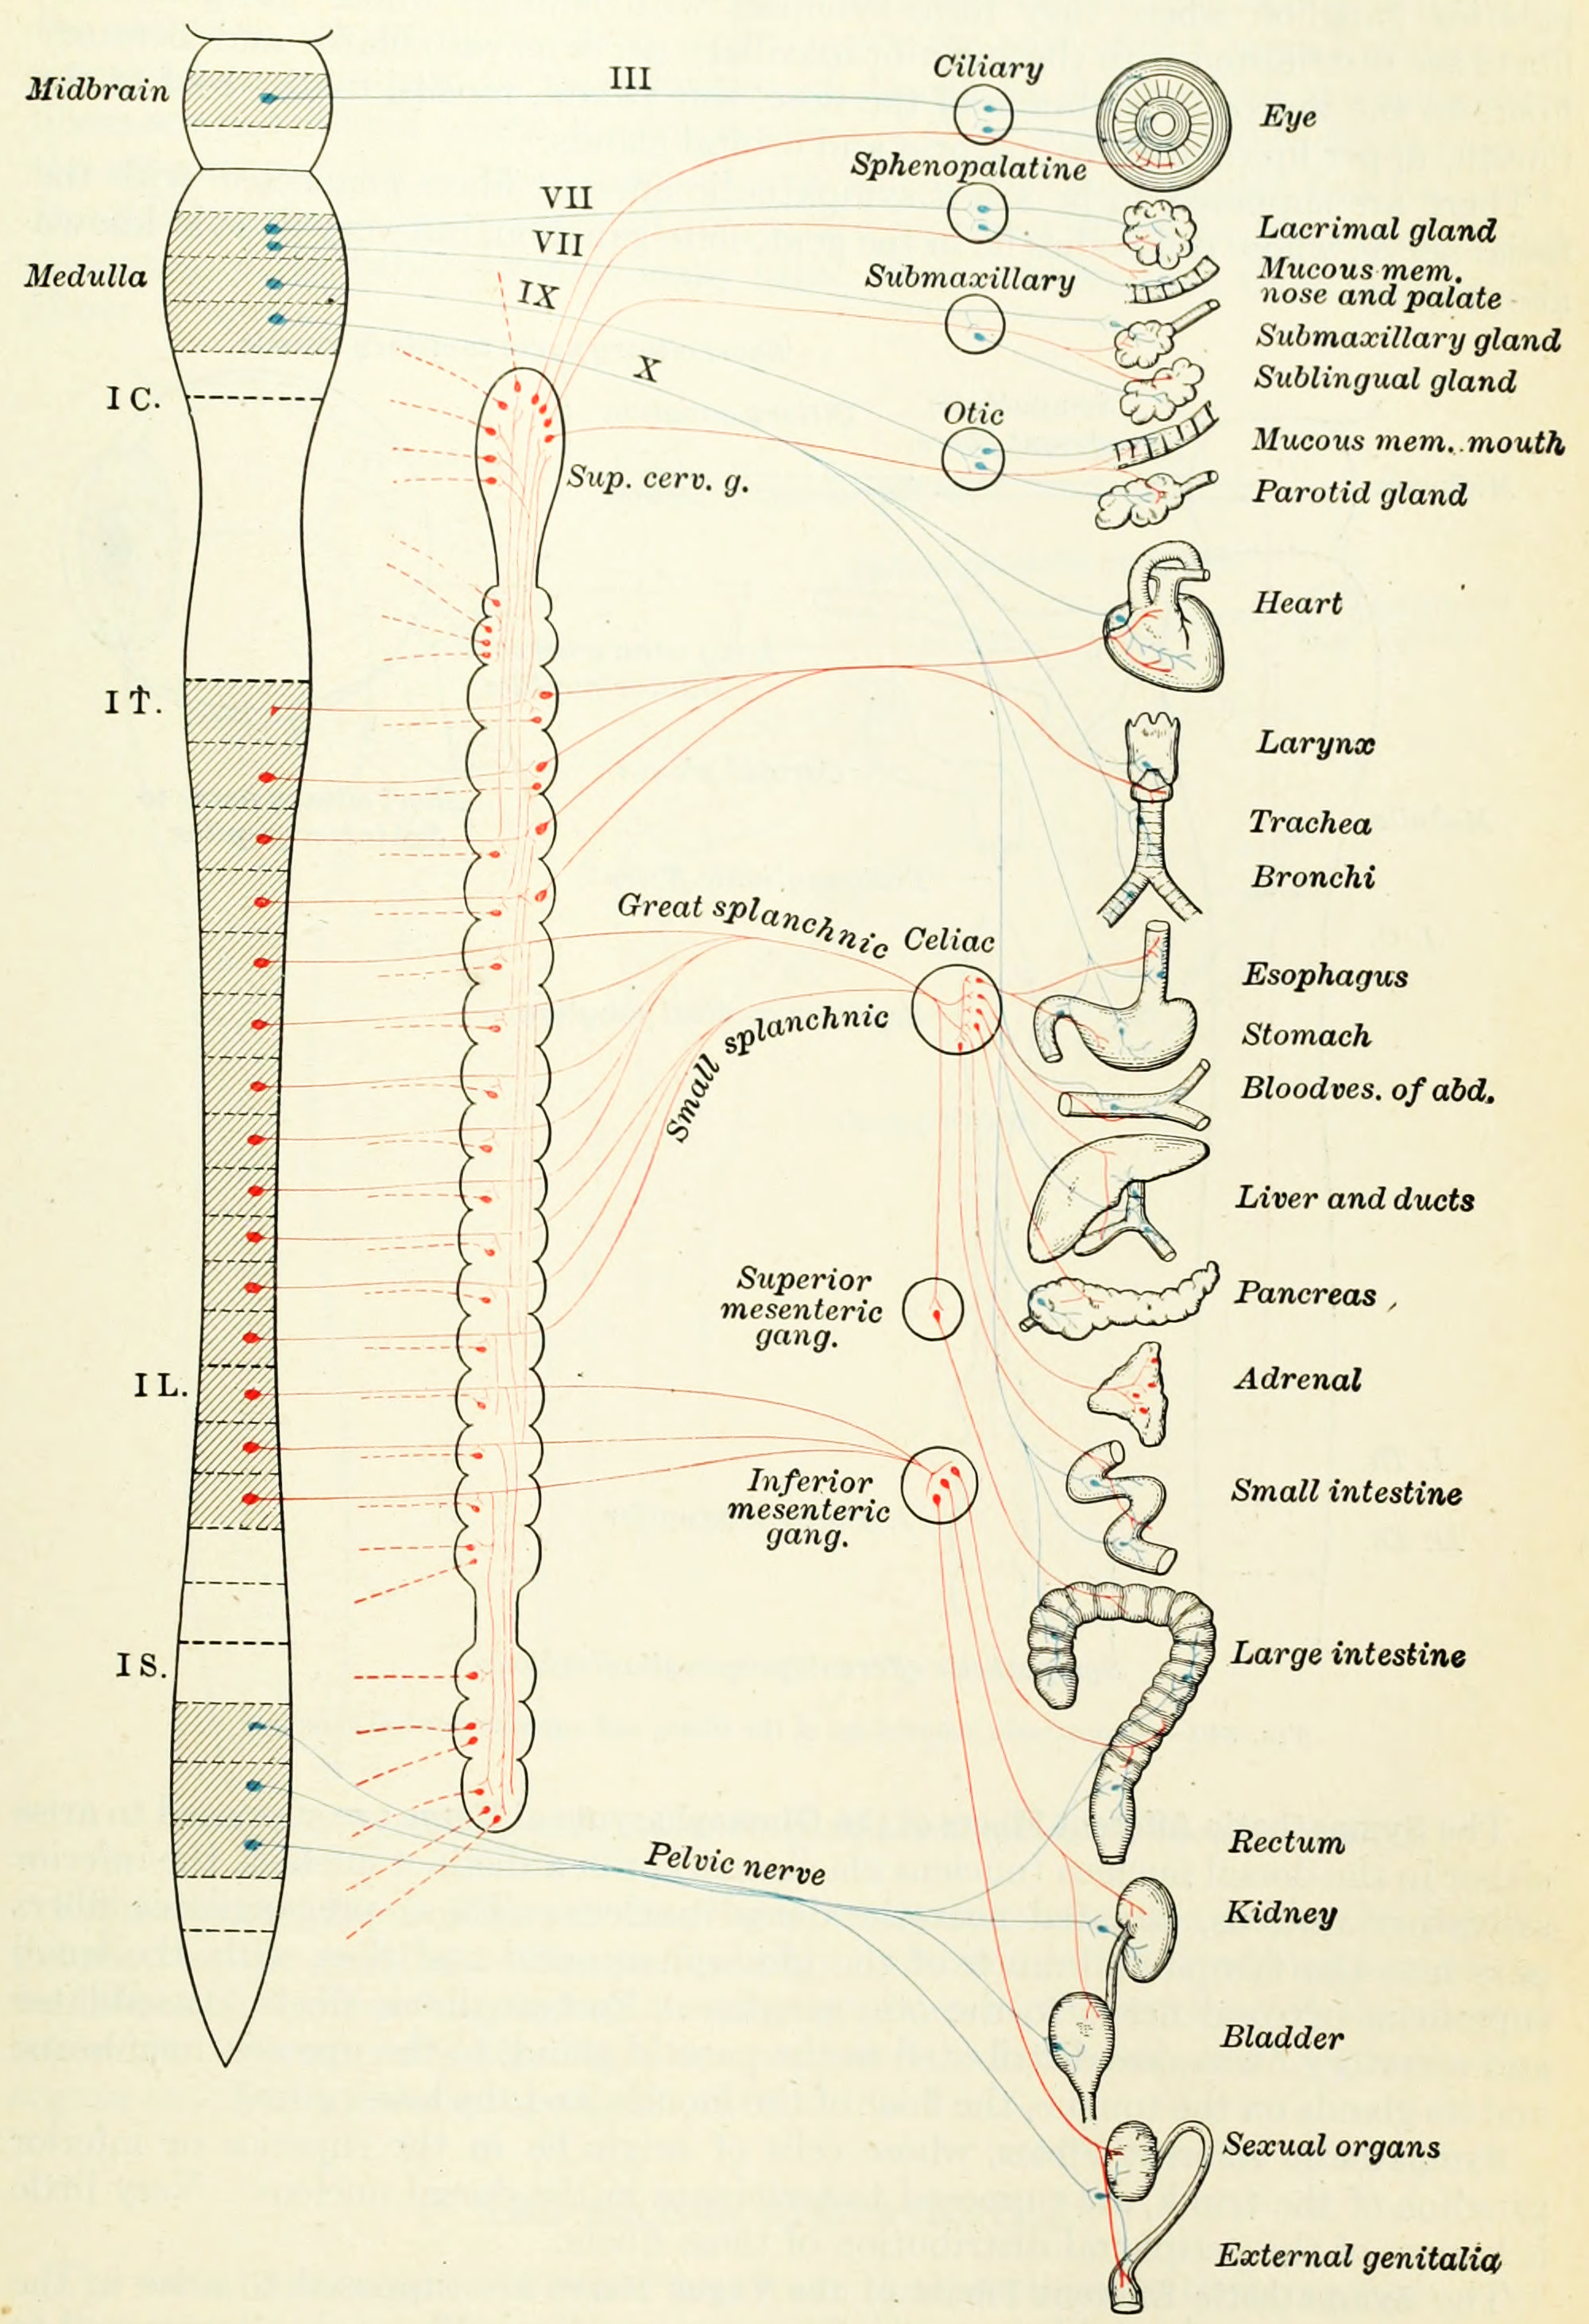
\includegraphics[width=0.7\linewidth]{./figures/pns/GrayAnat1918p971} 

}

\caption{Diagram of the sympathetic and parasympathetic divisions of the autonomic nervous system. Blue, cranial and sacral branches of the parasympathetic division. Red, the sympathetic division; broken lines(----), postganglionic fibers to spinal and cranial nerves to supply vasomotors to head, trunk and limbs, motor fibers to smooth muscles of skin and fibers to sweat glands. From \href{https://archive.org/details/anatomyofhumanbo1918gray/page/n6/mode/2up}{Gray Henry, Anatomy of the Human Body. 20\textsuperscript{th} Edition, Lea \& Febiger, Philadelphia \& New York, 1918}}\label{fig:autonomicdiagram}
\end{figure}

The autonomic nervous system is unique in that it requires a sequential two-neuron efferent pathway; the preganglionic neuron must first synapse onto a postganglionic neuron before innervating the target organ. The preganglionic, or first, neuron will begin at the ``outflow'' and will synapse at the postganglionic, or second, neuron's cell body. The postganglionic neuron will then synapse at the target organ.
\onecolumn
\begin{table}
\caption{\label{tab:autonomic}Effects of the parasympathetic and sympathetic branches of the autonomic system on their target organs.}
\begin{tabular}[t]{>{\raggedright\arraybackslash}p{10em}>{\raggedright\arraybackslash}p{20em}>{\raggedright\arraybackslash}p{25em}}
\toprule
Target organ/system & Parasympathetic & Sympathetic\\
\midrule
\rowcolor{gray!6}  Digestive system & Increase peristalsis and amount of secretion by digestive glands & Decrease activity of digestive system\\
Liver & No effect & Causes glucose to be release to blood\\
\rowcolor{gray!6}  Lungs & Constricts bronchioles & Dilates bronchioles\\
Urinary bladder/ Urethra & Relaxes sphincter & Constricts sphincter\\
\rowcolor{gray!6}  Kidneys & No effects & Decrease urine output\\
\addlinespace
Heart & Decreases rate & Increase rate\\
\rowcolor{gray!6}  Blood vessels & No effect on most blood vessels & Constricts blood vessels in viscera; increase BP\\
Salivary and Lacrimal glands & Stimulates; increases production of saliva and tears & Inhibits; result in dry mouth and dry eyes\\
\rowcolor{gray!6}  Eye (iris) & Stimulates constrictor muscles; constrict pupils & Stimulate dilator muscle; dilates pupils\\
Eye (ciliary muscles) & Stimulates to increase bulging of lens for close vision & Inhibits; decrease bulging of lens; prepares for distant vision\\
\addlinespace
\rowcolor{gray!6}  Adrenal Medulla & No effect & Stimulate medulla cells to secrete epinephrine and norepinephrine\\
Sweat gland of skin & No effect & Stimulate to produce perspiration\\
\bottomrule
\end{tabular}
\end{table}
\twocolumn
\hypertarget{the-sympathetic-nervous-system}{%
\section{The Sympathetic Nervous System}\label{the-sympathetic-nervous-system}}

The sympathetic nervous system is responsible for up- and down-regulating many homeostatic mechanisms in living organisms. Fibers from the SNS innervate tissues in almost every organ system, providing at least some regulation of functions as diverse as pupil diameter, gut motility, and urinary system output and function. It is perhaps best known for mediating the neuronal and hormonal stress response commonly known as the fight-or-flight response. This response is also known as sympatho-adrenal response of the body, as the preganglionic sympathetic fibers that end in the adrenal medulla (but also all other sympathetic fibers) secrete acetylcholine, which activates the great secretion of adrenaline (epinephrine) and to a lesser extent noradrenaline (norepinephrine) from it. Therefore, this response that acts primarily on the cardiovascular system is mediated directly via impulses transmitted through the sympathetic nervous system and indirectly via catecholamines secreted from the adrenal medulla.

The name of this system can be traced to the concept of sympathy, in the sense of ``connection between parts'', first used medically by Galen. In the 18th century, \href{https://en.wikipedia.org/wiki/Jacob_B._Winslow}{Jacob B. Winslow} applied the term specifically to nerves.

The sympathetic nervous system is responsible for priming the body for action, particularly in situations threatening survival. One example of this priming is in the moments before waking, in which sympathetic outflow spontaneously increases in preparation for action.

Sympathetic nervous system stimulation causes vasoconstriction of most blood vessels, including many of those in the skin, the digestive tract, and the kidneys. This occurs as a result of activation of alpha-1 adrenergic receptors by norepinephrine released by post-ganglionic sympathetic neurons. These receptors exist throughout the vasculature of the body but are inhibited and counterbalanced by beta-2 adrenergic receptors (stimulated by epinephrine release from the adrenal glands) in the skeletal muscles, the heart, the lungs, and the brain during a sympathoadrenal response. The net effect of this is a shunting of blood away from the organs not necessary to the immediate survival of the organism and an increase in blood flow to those organs involved in intense physical activity.

There are two kinds of neurons involved in the transmission of any signal through the sympathetic system: pre-ganglionic and post-ganglionic. The shorter preganglionic neurons originate in the thoracolumbar division of the spinal cord specifically at T1 to L2\textasciitilde L3, and travel to a ganglion, often one of the paravertebral ganglia, where they synapse with a postganglionic neuron. From there, the long postganglionic neurons extend across most of the body.

At the synapses within the ganglia, preganglionic neurons release acetylcholine, a neurotransmitter that activates nicotinic acetylcholine receptors on postganglionic neurons. In response to this stimulus, the postganglionic neurons release norepinephrine, which activates adrenergic receptors that are present on the peripheral target tissues. The activation of target tissue receptors causes the effects associated with the sympathetic system. However, there are three important exceptions:

\begin{enumerate}
\def\labelenumi{\arabic{enumi}.}
\tightlist
\item
  Postganglionic neurons of sweat glands release acetylcholine for the activation of muscarinic receptors, except for areas of thick skin, the palms and the plantar surfaces of the feet, where norepinephrine is released and acts on adrenergic receptors.
\item
  Chromaffin cells of the adrenal medulla are analogous to post-ganglionic neurons; the adrenal medulla develops in tandem with the sympathetic nervous system and acts as a modified sympathetic ganglion. Within this endocrine gland, pre-ganglionic neurons synapse with chromaffin cells, triggering the release of two transmitters: a small proportion of norepinephrine, and more substantially, epinephrine. The synthesis and release of epinephrine as opposed to norepinephrine is another distinguishing feature of chromaffin cells compared to postganglionic sympathetic neurons.
\item
  Postganglionic sympathetic nerves terminating in the kidney release dopamine, which acts on dopamine D1 receptors of blood vessels to control how much blood the kidney filters. Dopamine is the immediate metabolic precursor to norepinephrine, but is nonetheless a distinct signaling molecule.
\end{enumerate}

Sympathetic nerves arise from near the middle of the spinal cord in the intermediolateral nucleus of the lateral grey column, beginning at the first thoracic vertebra of the vertebral column and are thought to extend to the second or third lumbar vertebra. Because its cells begin in the thoracolumbar division -- the thoracic and lumbar regions of the spinal cord, the sympathetic nervous system is said to have a thoracolumbar outflow. Axons of these nerves leave the spinal cord through the anterior root. They pass near the spinal (sensory) ganglion, where they enter the anterior rami of the spinal nerves. However, unlike somatic innervation, they quickly separate out through white rami connectors (so called from the shiny white sheaths of myelin around each axon) that connect to either the paravertebral (which lie near the vertebral column) or prevertebral (which lie near the aortic bifurcation) ganglia extending alongside the spinal column.

Presynaptic nerves' axons terminate in either the paravertebral ganglia or prevertebral ganglia. There are four different paths an axon can take before reaching its terminal. In all cases, the axon enters the paravertebral ganglion at the level of its originating spinal nerve. After this, it can then either synapse in this ganglion, ascend to a more superior or descend to a more inferior paravertebral ganglion and synapse there, or it can descend to a prevertebral ganglion and synapse there with the postsynaptic cell.

The postsynaptic cell then goes on to innervate the targeted end effector (i.e.~gland, smooth muscle, etc.). Because paravertebral and prevertebral ganglia are relatively close to the spinal cord, presynaptic neurons are generally much shorter than their postsynaptic counterparts, which must extend throughout the body to reach their destinations.

A notable exception to the routes mentioned above is the sympathetic innervation of the suprarenal (adrenal) medulla. In this case, presynaptic neurons pass through paravertebral ganglia, on through prevertebral ganglia and then synapse directly with suprarenal tissue. This tissue consists of cells that have pseudo-neuron like qualities in that when activated by the presynaptic neuron, they will release their neurotransmitter (epinephrine) directly into the bloodstream.

\hypertarget{the-parasympathetic-nervous-system}{%
\section{The Parasympathetic Nervous System}\label{the-parasympathetic-nervous-system}}

The parasympathetic system is responsible for stimulation of ``rest-and-digest'' or ``feed and breed'' activities that occur when the body is at rest, especially after eating, including sexual arousal, salivation, lacrimation (tears), urination, digestion and defecation. Its action is described as being complementary to that of the sympathetic nervous system, which is responsible for stimulating activities associated with the fight-or-flight response.

Nerve fibres of the parasympathetic nervous system arise from the central nervous system. Specific nerves include several cranial nerves, specifically the oculomotor nerve, facial nerve, glossopharyngeal nerve, and vagus nerve. Three spinal nerves in the sacrum (S2-4), commonly referred to as the pelvic splanchnic nerves, also act as parasympathetic nerves.

The parasympathetic nervous system uses chiefly acetylcholine (ACh) as its neurotransmitter, although peptides (such as cholecystokinin) can be used. The ACh acts on two types of receptors, the muscarinic and nicotinic cholinergic receptors. Most transmissions occur in two stages: When stimulated, the preganglionic neuron releases ACh at the ganglion, which acts on nicotinic receptors of postganglionic neurons. The postganglionic neuron then releases ACh to stimulate the muscarinic receptors of the target organ.

Owing to its location, the parasympathetic system is commonly referred to as having ``craniosacral outflow'', which stands in contrast to the sympathetic nervous system, which is said to have ``thoracolumbar outflow''.

The parasympathetic nerves are autonomic or visceral  branches of the peripheral nervous system (PNS). Parasympathetic nerve supply arises through three primary areas:

\begin{enumerate}
\def\labelenumi{\arabic{enumi}.}
\tightlist
\item
  Certain cranial nerves in the cranium, namely the preganglionic parasympathetic nerves (CN III, CN VII, and CN IX) usually arise from specific nuclei in the central nervous system (CNS) and synapse at one of four parasympathetic ganglia: ciliary, pterygopalatine, otic, or submandibular. From these four ganglia the parasympathetic nerves complete their journey to target tissues via trigeminal branches (ophthalmic nerve, maxillary nerve, mandibular nerve).
\item
  The vagus nerve does not participate in these cranial ganglia as most of its parasympathetic fibers are destined for a broad array of ganglia on or near thoracic viscera (esophagus, trachea, heart, lungs) and abdominal viscera (stomach, pancreas, liver, kidneys, small intestine, and about half of the large intestine). The vagus innervation ends at the junction between the midgut and hindgut, just before the splenic flexure of the transverse colon.
\item
  The pelvic splanchnic efferent preganglionic nerve cell bodies reside in the lateral gray horn of the spinal cord at the T12-L1 vertebral levels (the spinal cord terminates at the L1-L2 vertebrae with the conus medullaris), and their axons exit the vertebral column as S2-S4 spinal nerves through the sacral foramina. Their axons continue away from the CNS to synapse at an autonomic ganglion. The parasympathetic ganglion where these preganglionic neurons synapse will be close to the organ of innervation. This differs from the sympathetic nervous system, where synapses between pre- and post-ganglionic efferent nerves in general occur at ganglia that are farther away from the target organ.
\end{enumerate}

As in the sympathetic nervous system, efferent parasympathetic nerve signals are carried from the central nervous system to their targets by a system of two neurons. The first neuron in this pathway is referred to as the preganglionic or presynaptic neuron. Its cell body sits in the central nervous system and its axon usually extends to synapse with the dendrites of a postganglionic neuron somewhere else in the body. The axons of presynaptic parasympathetic neurons are usually long, extending from the CNS into a ganglion that is either very close to or embedded in their target organ. As a result, the postsynaptic parasympathetic nerve fibers are very short.

The oculomotor nerve is responsible for a number of parasympathetic functions related to the eye. The oculomotor PNS fibers originate in the Edinger-Westphal nucleus in the central nervous system and travel through the superior orbital fissure to synapse in the ciliary ganglion located just behind the orbit (eye). From the ciliary ganglion the postganglionic parasympathetic fibers leave via short ciliary nerve fibers, a continuation of the nasociliary nerve (a branch of ophthalmic division of the trigeminal nerve (CN V1)). The short ciliary nerves innervate the orbit to control the ciliary muscle (responsible for accommodation) and the iris sphincter muscle, which is responsible for miosis or constriction of the pupil (in response to light or accommodation). There are two motors that are part of the oculomotor nerve known as the somatic motor and visceral motor. The somatic motor is responsible for moving the eye in precise motions and for keeping the eye fixated on an object. The visceral motor helps constrict the pupil.

The parasympathetic aspect of the facial nerve controls secretion of the sublingual and submandibular salivary glands, the lacrimal gland, and the glands associated with the nasal cavity. The preganglionic fibers originate within the CNS in the superior salivatory nucleus and leave as the intermediate nerve (which some consider a separate cranial nerve altogether) to connect with the facial nerve just distal (further out) to it surfacing the central nervous system. Just after the facial nerve geniculate ganglion (general sensory ganglion) in the temporal bone, the facial nerve gives off two separate parasympathetic nerves. The first is the greater petrosal nerve and the second is the chorda tympani. The greater petrosal nerve travels through the middle ear and eventually combines with the deep petrosal nerve (sympathetic fibers) to form the nerve of the pterygoid canal. The parasympathetic fibers of the nerve of the pterygoid canal synapse at the pterygopalatine ganglion, which is closely associated with the maxillary division of the trigeminal nerve (CN V2). The postganglionic parasympathetic fibers leave the pterygopalatine ganglion in several directions. One division leaves on the zygomatic division of CN V2 and travels on a communicating branch to unite with the lacrimal nerve (branch of the ophthalmic nerve of CN V1) before synapsing at the lacrimal gland. These parasympathetic to the lacrimal gland control tear production.

A separate group of parasympathetic leaving from the pterygopalatine ganglion are the descending palatine nerves (CN V2 branch), which include the greater and lesser palatine nerves. The greater palatine parasympathetic synapse on the hard palate and regulate mucus glands located there. The lesser palatine nerve synapses at the soft palate and controls sparse taste receptors and mucus glands. Yet another set of divisions from the pterygopalatine ganglion are the posterior, superior, and inferior lateral nasal nerves; and the nasopalatine nerves (all branches of CN V2, maxillary division of the trigeminal nerve) that bring parasympathetic innervation to glands of the nasal mucosa. The second parasympathetic branch that leaves the facial nerve is the chorda tympani. This nerve carries secretomotor fibers to the submandibular and sublingual glands. The chorda tympani travels through the middle ear and attaches to the lingual nerve (mandibular division of trigeminal, CN V3). After joining the lingual nerve, the preganglionic fibers synapse at the submandibular ganglion and send postganglionic fibers to the sublingual and submandibular salivary glands.

The glossopharyngeal nerve has parasympathetic fibers that innervate the parotid salivary gland. The preganglionic fibers depart CN IX as the tympanic nerve and continue to the middle ear where they make up a tympanic plexus on the cochlear promontory of the mesotympanum. The tympanic plexus of nerves rejoin and form the lesser petrosal nerve and exit through the foramen ovale to synapse at the otic ganglion. From the otic ganglion postganglionic parasympathetic fibers travel with the auriculotemporal nerve (mandibular branch of trigeminal, CN V3) to the parotid salivary gland.

The vagus nerve, named after the Latin word vagus (because the nerve controls such a broad range of target tissues -- vagus in Latin literally means ``wandering''), has parasympathetic functions that originate in the dorsal nucleus of the vagus nerve and the nucleus ambiguus in the CNS. The vagus nerve is an unusual cranial parasympathetic in that it doesn't join the trigeminal nerve in order to get to its target tissues. Another peculiarity is that the vagus has an autonomic ganglion associated with it at approximately the level of C1 vertebra. The vagus gives no parasympathetic to the cranium. The vagus nerve is hard to track definitively due to its ubiquitous nature in the thorax and abdomen so the major contributions will be discussed. Several parasympathetic nerves come off the vagus nerve as it enters the thorax. One nerve is the recurrent laryngeal nerve, which becomes the inferior laryngeal nerve. From the left vagus nerve the recurrent laryngeal nerve hooks around the aorta to travel back up to the larynx and proximal esophagus while, from the right vagus nerve, the recurrent laryngeal nerve hooks around the right subclavian artery to travel back up to the same location as its counterpart. These different paths are a direct result of embryological development of the circulatory system. Each recurrent laryngeal nerve supplies the trachea and the esophagus with parasympathetic secretomotor innervation for glands associated with them (and other fibers that are not PN).

Another nerve that comes off the vagus nerves approximately at the level of entering the thorax are the cardiac nerves. These cardiac nerves go on to form cardiac and pulmonary plexuses around the heart and lungs. As the main vagus nerves continue into the thorax they become intimately linked with the esophagus and sympathetic nerves from the sympathetic trunks to form the esophageal plexus. This is very efficient as the major function of the vagus nerve from there on will be control of the gut smooth muscles and glands. As the esophageal plexus enter the abdomen through the esophageal hiatus anterior and posterior vagus trunks form. The vagus trunks then join with preaortic sympathetic ganglion around the aorta to disperse with the blood vessels and sympathetic nerves throughout the abdomen. The extent of the parasympathetic in the abdomen include the pancreas, kidneys, liver, gall bladder, stomach and gut tube. The vagus contribution of parasympathetic continues down the gut tube until the end of the midgut. The midgut ends two thirds of the way across the transverse colon near the splenic flexure.

The vagus nerve plays a crucial role in heart rate regulation by modulating the response of sinoatrial node.

The pelvic splanchnic nerves, S2-4, work in tandem to innervate the pelvic viscera. Unlike in the cranium, where one parasympathetic is in charge of one particular tissue or region, for the most part the pelvic splanchnics each contribute fibers to pelvic viscera by traveling to one or more plexuses before being dispersed to the target tissue. These plexuses are composed of mixed autonomic nerve fibers (parasympathetic and sympathetic) and include the vesical, prostatic, rectal, uterovaginal, and inferior hypogastric plexuses. The preganglionic neurons in the pathway do not synapse in a ganglion as in the cranium but rather in the walls of the tissues or organs that they innervate. The fiber paths are variable and each individual's autonomic nervous system in the pelvis is unique. The visceral tissues in the pelvis that the parasympathetic nerve pathway controls include those of the urinary bladder, ureters, urinary sphincter, anal sphincter, uterus, prostate, glands, vagina, and penis. Unconsciously, the parasympathetic will cause peristaltic movements of the ureters and intestines, moving urine from the kidneys into the bladder and food down the intestinal tract and, upon necessity, the parasympathetic will assist in excreting urine from the bladder or defecation. Stimulation of the parasympathetic will cause the detrusor muscle (urinary bladder wall) to contract and simultaneously relax the internal sphincter muscle between the bladder and the urethra, allowing the bladder to void. Also, parasympathetic stimulation of the internal anal sphincter will relax this muscle to allow defecation. There are other skeletal muscles involved with these processes but the parasympathetic plays a huge role in continence and bowel retention.

Another role that the parasympathetic nervous system plays is in sexual activity. In males, the cavernous nerves from the prostatic plexus stimulate smooth muscles in the fibrous trabeculae of the coiled helicine arteries of penis to relax and allow blood to fill the two corpora cavernosa and the corpus spongiosum of the penis, making it rigid to prepare for sexual activity. Upon emission of ejaculate, the sympathetics participate and cause peristalsis of the ductus deferens and closure of the internal urethral sphincter to prevent semen from entering the bladder. At the same time, parasympathetics cause peristalsis of the urethral muscle, and the pudendal nerve causes contraction of the bulbospongiosus to forcibly emit the semen. During remission the penis becomes flaccid again. In the female, there is erectile tissue analogous to the male yet less substantial that plays a large role in sexual stimulation. The PN cause release of secretions in the female that decrease friction. Also in the female, the parasympathetics innervate the fallopian tubes, which helps peristaltic contractions and movement of the oocyte to the uterus for implantation. The secretions from the female genital tract aid in sperm migration.


